\chapter{Experiment and Results}
In this chapter, section 4.1 describe component of database used in experiment, and section 4.2 introduce methodologies of classification and evaluation. Section 4.3 presents the result and give explanation of analysis.
\section{Data}
There are 450 videos in two formats, avi and flv, 89 of them are flv videos, 361 of them are avi videos. The time of videos are from seconds to dozens of seconds. Videos were recorded using web-cam of different PCs. Video background are vary as the video are recorded in a place chosen by subject. People are free to do anything while recording the video, a male disappear from the camera for half of the video sequence while recording. As a result, there are no faces in most of the video frames. The Intraface tracker \cite{xiong2013supervised} is used to track those videos. It is able to track 439 videos. 1 video is tracked, but the tracking result does not match the label. 10 videos are tracked, but unable to identify the face in the video. The face in those untracked video can be clear identify by visual. One possible may be the resolution of the image. Maximum untracked video frame is $240*960$ pixels. Minimum tracked video frame size is $240*960$, the same as the maximum size of untracked video frame. It is reasonable to say tracker \cite{xiong2013supervised} may not be good at tracking low resolution videos. The observation mentioned in comparing tracker \cite{xiong2013supervised} and tracker \cite{asthana2013robust} also support this hypothesis. The maximum frame tracked is $600*2400$. For each video there is a label file indicate the label of each frame, The frame number of each video is quite different, from around 200 to more than 900. The frame rate is 30 fps. Table\ref{tab:TR} shows the tracking result of tracker \cite{xiong2013supervised}.
\begin{table}[ht]
\begin{tabular}{|l|*{6}{c|}}
\hline
\diagbox{Title}{Label} & Normal Face & Eating & Talking & Looking Away & Occluded & Other Problem \\ \hline
Total   & 35361       & 10409  & 5623    & 7730         & 21394    & 8422          \\ \hline
Tracked & 33776       & 9460   & 5196    & 5405         & 19014    & 3884          \\ \hline   
Rate		& 0.9552      & 0.9088 & 0.9241  & 0.6992       & 0.8888   & 0.4612        \\ \hline
\end{tabular}
\caption{Frame tracking result by tracker \cite{xiong2013supervised}}
\label{tab:TR}
\end{table}
\newline
There are six labels for each frame, normal face, eating, talking, looking away, occluded, other problem. A frame labelled as eating belong to a image sequence of eating. Label normal face, eating, talking and looking away are disjoint, but one frame can be labelled as one of them and occluded or other problem. It is very hard to track a face that face to camera from a certain angle, so the tracking rate is very small for a face looking away. Only frame with label normal face, eating, talking in the experiment. Not all three labels are included in all videos, most of videos miss one or two or even all three labels.
\newline
The three class: Normal Face, Eating, Talking are used for training and classification. The statistical data are show in table \ref{tab:UFD} and \ref{tab:USD}.
\begin{table}[ht]
\centering
\begin{tabular}{l|l|l|l|}
\cline{2-4}
                                                   & Normal Face & Eating & Talking \\ \hline
\multicolumn{1}{|l|}{Tracked Frame Number}         & 33776       & 9460   & 5196    \\ \hline
\multicolumn{1}{|l|}{Percentage of this class}     & 0.6974      & 0.1953 & 0.1073  \\ \hline
\multicolumn{1}{|l|}{Percentage of not this class} & 0.3026      & 0.8047 & 0.8927  \\ \hline
\end{tabular}
\caption{Extracted Frames of Normal Face, Eating, Talking}
\label{tab:UFD}
\end{table}
\begin{table}[ht]
\centering
\begin{tabular}{l|l|l|l|}
\cline{2-4}
                                                   & Normal Face & Eating & Talking \\ \hline
\multicolumn{1}{|l|}{Tracked Sequence Number}      & 871         & 114    & 207     \\ \hline
\multicolumn{1}{|l|}{Percentage of this class}     & 0.7307      & 0.0956 & 0.1737  \\ \hline
\multicolumn{1}{|l|}{Percentage of not this class} & 0.2693      & 0.9044 & 0.8263  \\ \hline
\end{tabular}
\caption{Extracted Sequences of Normal Face, Eating, Talking}
\label{tab:USD}
\end{table}
\subsection{Feature}
Each face is aligned with 49 facial feature points as shown in figure \ref{fig:IPI}. As the tracker doesn't provide face bound point,so it's not possible to include jaw and cheek in the ROI.  Only the mouth as Region of Interest. Then Local Binary Pattern feature is extracted from ROI. The size appearance feature vector are different if image of ROI is divided into different number of blocks. 1 block and $1*3$ blocks are tried on dividing the image, the size of appearance feature vector is 95 and 177. As there are 49 shape feature points, so the size of shape feature points is 98.
\section{Methodology}
In the classification part, Support Vector Machine for classification. Two different type of appearance feature vectors are experimented, their dimensionality is 95 and 177, to see whether with more detailed appearance feature vector would be better for classification. The experiment focusing on finding answers to two question, would divide the image into more blocks while using LBP to extract features would influence the classification result, whether apply normalisation to each video would improve the classification result. In order to answer the first question, two group of features are examined. Both of them are extracted using blocked uniform pattern. However, one divides the image into 3 blocks, the other treats the image as one block. In order to find the answer to the second question, two different process are applied in normalising the features vector, one normalises both appearance feature and shape feature by each video, the other does not. One thing need mentions is that after put all feature vector together, feature vector of all groups are normalised. There are three types of feature vectors: shape feature vector, appearance feature vector and appearance+shape feature vector. As extracting feature using blocked uniform pattern only affect appearance feature vector, so in total, there are 10 groups of experiments.

SVM are fistly tested with linear kernel function and non-linear kernel, the Gaussian Kernel shows better result. Gaussian and polynomial kernels often leads to over-fitting in high dimensional database, while linear kernel is easier to tune because the only parameter that affects performance is the soft-margin constant\cite{ben2010user}. The best result is using Gaussian Kernel, so Gaussian Kernel is used for classification. The most important parameters for Gaussian Kernel is  penalty parameter $c$ and $\gamma$ in equation \ref{eq:GK}. Find the proper parameter could significantly increase classification result.\begin{equation}
K(x,x') = e^{-\gamma||x-x'||^{2}}
\label{eq:GK}
\end{equation}

\subsection{Dealing with imbalanced data}
We tried several actions to reduce the influence of imbalanced problem.
\begin{itemize}
\item Use 10-fold cross validation to all the classification result for all the entities. 
\item According to the number of training entities of each class, tune the training weight of each class.
\item Or for each training, random select approximately the same number of entities in each class, usually .
\end{itemize}
\subsection{libSVM}
libSVM uses 'one-against-one' approach for multi-class classification\cite{CC01a}. If there are $n$ different classes, it will generate $n(n-1)/2$ classifier, each classifier is trained with two classes. It also use a voting strategy: each entity is test with each classifier, the entity belong to the class with most number of votes.
\subsection{Parameter Optimisation for SVM}
A general way to find parameter $c$ and $\gamma$ is using cross-validation and grid-search. In n-fold cross-validation, first equally divide the data into n fold, leave out one fold of data as testing data and use other $n-1$ fold of data to train the classifier. Thus all the data is predicted once and the cross-validation accuracy is the percentage of data are correctly classified. 
Grid-search is try various pairs of $c$ and $\gamma$ and choose the one with best cross-validation accuracy. Grid search approach is very simply and the computational time is no more than advanced method. To shorten the time of grid search, it is better to search with a coarse grid and then proceed with a more specific search in the identified grid.
\subsection{Evaluation}
In order to compare the different classification result, precision rate, recall rate and F measure to evaluate classification result of each group of data. For each class could form a table of 2x2 and 4 result, true position(TP), true negative(TN), false positive(FP), false negative(FN) as shown in table.
\begin{table}[ht]
\centering
\begin{tabular}{ll|l|l|}
\cline{3-4}
\multicolumn{2}{l}{\multirow{2}{*}{}}                                                                  & \multicolumn{2}{|l|}{Predicted Class} \\ \cline{3-4} 
\multicolumn{2}{l|}{}                                                                                   & Class             & Other            \\ \hline
\multicolumn{1}{|l|}{\multirow{2}{*}{\begin{tabular}[c]{@{}l@{}}Actual\\ Class\end{tabular}}} & Class & TP                & FN               \\ \cline{2-4} 
\multicolumn{1}{|l|}{}                                                                         & Other & FP                & TN               \\ \hline
\end{tabular}
\caption{Confusion Matrix for two class}
\label{tab:CM-2}
\end{table}
\newline
Recall rate is the percentage of actual entities that are correctly Predicted Positive\cite{powers2011evaluation}. Precision rate is the percentage of Predicted Positive entities that are correctly real positives\cite{powers2011evaluation}. TP represents the number of positives are correctly classified. FN represents the number of negatives are false classified. FP represents the number of positives are false classified. TN represents the number of negatives that are correctly classified. F measure evaluates both recall rate and precision rate. In this experiment, F1 measure are used for evaluation the result. The best score for F1 measure is 1 and the worst is 0, it can be interpreted as average weighted recall rate and precision rate.
\begin{equation}
\begin{split}
recall &= \frac{TP}{TP + FN} \times 100\% \\
precision &= \frac{TP}{TP+FP} \times 100\% \\
F_{\alpha} &= (1+\alpha)\frac{precision*recall}{\alpha*precision+recall}
\end{split} 
\end{equation}

\section{Experiments}
In this chapter, a detail description of results and explanations of analysis are presented. Figure \ref{fig:REF}, \ref{fig:RTF}, \ref{fig:RNF}, are frame classification result of Class Eating, Talking, Normal Face, using feature vectors that are normalised by each video. Figure \ref{fig:REF1}, \ref{fig:RTF1}, \ref{fig:RNF1}, are frame classification result of Class Eating, Talking, Normal Face, using feature vectors that are NOT normalised by each video. Figure \ref{fig:RES}, \ref{fig:RTS}, \ref{fig:RNS}, are sequence classification result of Class Eating, Talking, Normal Face, using feature vectors that are normalised by each video. Figure \ref{fig:RES1}, \ref{fig:RTS1}, \ref{fig:RNS1}, are sequence classification result of Class Eating, Talking, Normal Face, using feature vectors that are NOT normalised by each video. Figure \ref{fig:RNF}, \ref{fig:RFS} are frame and sequence F1 measure of all three class using feature vectors that are normalised by each video. Figure \ref{fig:RFF1}, \ref{fig:RFS1} are frame and sequence F1 measure of all three class using feature vectors that are NOT normalised by each video.

Most figure contains result of 5 groups, 1\_A means the appearance feature is extracted by using 1 block uniform pattern and it is using appearance vector for classification. 3\_AS means the appearance feature is extracted by using 3 block uniform pattern and it is using appearance and shape vector for classification. The same for 1\_AS and 3\_A, as using pure shape feature vector, it is not marked as normalised or not normalised. The identification of each group of classification is show in table \ref{tab:RID}.
\begin{table}[ht]
\centering
\begin{tabular}{|l|*{11}{c|}}
\hline
\begin{tabular}[c]{@{}l@{}}Identification\end{tabular} & 1\_A & 1\_AS & 3\_A & 3\_AS & S   & S\_1   & 1\_A\_1 & 1\_AS\_1 & 3\_A\_1 & 3\_AS\_1 \\ \hline
\begin{tabular}[c]{@{}l@{}}Normalisation\\ (True if By Video)\end{tabular}            & T & T   & T & T   & T   & F   & F & F   & F & F   \\ \hline
\begin{tabular}[c]{@{}l@{}}Appearance Feature\\ (1 or 3 Block)\end{tabular} & 1 & 1   & 3 & 3   & 1/3 & 1/3 & 1 & 1   & 3 & 3   \\ \hline
\begin{tabular}[c]{@{}l@{}}Feature\\ A: Appearance\\ S: Shape\end{tabular}            & A & A+S & A & A+S & S   & S   & A & A+S & A & A+S \\ \hline
\end{tabular}
\caption{Experiments and Identification in result figure}
\label{tab:RID}
\end{table}

\subsection{Results and Analysis}
\begin{figure}[ht]
\centering
\begin{minipage}{.5\textwidth}
  \centering
  \captionsetup{justification=centering,margin=1cm}
  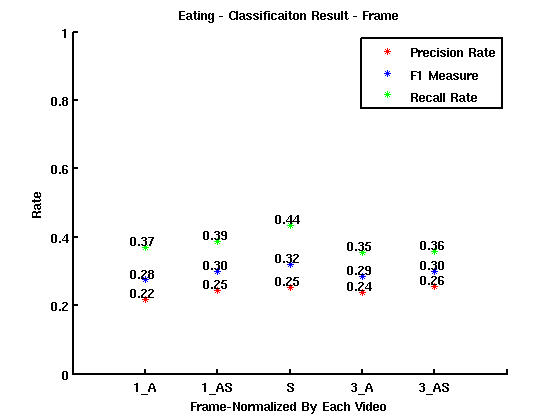
\includegraphics[width=\linewidth]{imgs/Result_Eating_Frame.png}
  \caption{Class Eating - Classification Result of Frame - Frame normalised by each video}
  \label{fig:REF}
\end{minipage}%
\begin{minipage}{.5\textwidth}
  \centering
  \captionsetup{justification=centering,margin=1cm}
  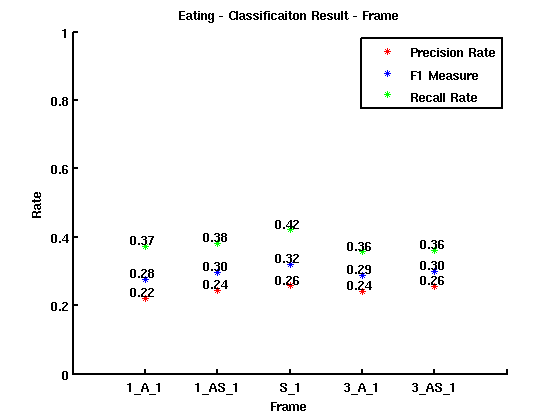
\includegraphics[width=\linewidth]{imgs/Result_Eating_Frame_1.png}
  \caption{Class Eating - Classification Result of Frame - Frame NOT normalised by each video}
  \label{fig:REF1}
\end{minipage}
\end{figure}
Figure \ref{fig:REF} shows precision rate, recall rate and F1 score of using appearance feature vector that are normalised by each video. The largest recall rate and F1 score are obtained by using shape feature vector in figure \ref{fig:REF} and \ref{fig:REF1}, which means shape feature is very good for classifying eating. The lowest F1 score is obtained by using 1-block appearance feature vector. For F1 score, 3\_A is better than 1\_A and 3\_AS is better than 1\_AS may because using using 3-block LBP provides more information mouth region. The average F1 score of figure \ref{fig:REF} is 0.3, almost the same figure \ref{fig:REF1}, means normalise each feature vector of each video does not influence performance of classification eating. F1 score of both figure are in the range of 0.3$\pm$0.02, it is very close, it may means there is not much difference of using appearance feature or shape feature or both for classification. In addition,  average score of classifying eating is 0.3, personally hypothesis is that distinguish eating from talking may be difficult. 
\begin{figure}[ht]
\centering
\begin{minipage}{.5\textwidth}
  \centering
  \captionsetup{justification=centering,margin=1cm}
  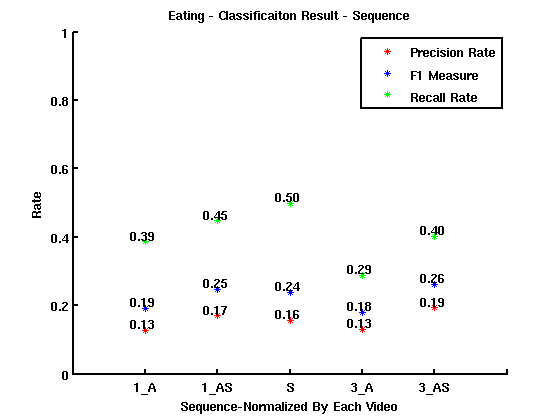
\includegraphics[width=\linewidth]{imgs/Result_Eating_Sequence.png}
  \caption{Class Eating - Classification Result of Sequence - Sequence normalised by each video}
  \label{fig:RES}
\end{minipage}%
\begin{minipage}{.5\textwidth}
  \centering
  \captionsetup{justification=centering,margin=1cm}
  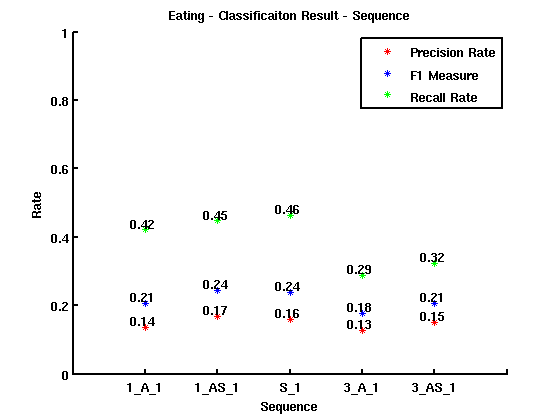
\includegraphics[width=\linewidth]{imgs/Result_Eating_Sequence_1.png}
  \caption{Class Eating - Classification Result of Sequence - Sequence NOT normalised by each video}
  \label{fig:RES1}
\end{minipage}
\end{figure}
\newline
Figure \ref{fig:RES} and \ref{fig:REF1} shows the sequence classification result of eating. In figure \ref{fig:RES} comparing to figure \ref{fig:REF}, there is a significant increase on recall rate of 1\_AS, 1\_S and 3\_AS, and there is a significant drop of precision rate and F1 score, it may because as percentage of eating class number drop from approximate 0.2 of frames to 0.1 of sequences.  The average of F1 score are almost the same for figure \ref{fig:REF} and \ref{fig:REF1} which the same situation as frame classification. However, the best F1 score is obtained by 3\_AS if figure \ref{fig:REF} and by S in figure \ref{fig:REF1}. In figure \ref{fig:RES} and \ref{fig:RES1} the average F1 scores are 0.224 and 0.216, standard deviation of F1 score in figure \ref{fig:REF} is 0.0365 and standard deviation of F1 score in figure \ref{fig:REF1} is 0.0251, this means in classifying eating although not normalising data by video may lead to a little less in classification performance the result of using different feature vector could be more stable.
\begin{figure}[ht]
\centering
\begin{minipage}{.5\textwidth}
  \centering
  \captionsetup{justification=centering,margin=1cm}
  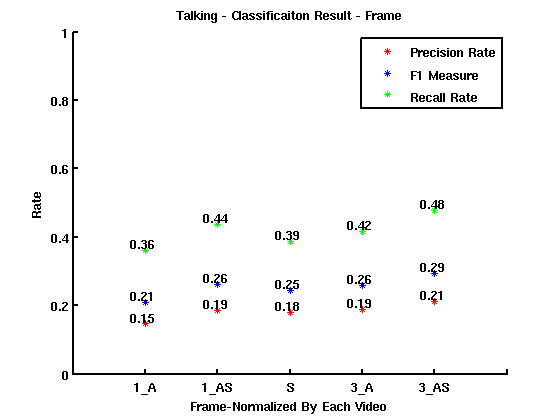
\includegraphics[width=\linewidth]{imgs/Result_Talking_Frame.png}
  \caption{Class Talking - Classification Result of Frame - Frame normalised by each video}
  \label{fig:RTF}
\end{minipage}%
\begin{minipage}{.5\textwidth}
  \centering
  \captionsetup{justification=centering,margin=1cm}
  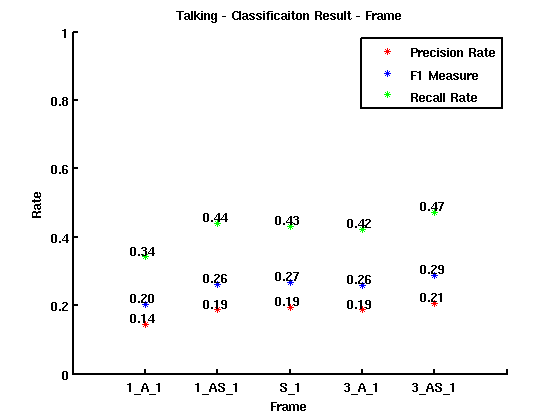
\includegraphics[width=\linewidth]{imgs/Result_Talking_Frame_1.png}
  \caption{Class Talking - Classification Result of Frame - Frame NOT normalised by each video}
  \label{fig:RTF1}
\end{minipage}
\end{figure}
\newline
In figure \ref{fig:RTF}, the best F1 score is obtained by 3\_AS, unlike figure \ref{fig:REF}, best F1 score is obtained by S. In addition, F1 score of 1\_AS  is better than S in figure \ref{fig:RTF}, which is different as in figure \ref{fig:REF} F1 score of S is better than 1\_AS. What's more, F1 score of those classification using both appearance and shape feature are larger than others, and it is the same result for figure \ref{fig:RTF1}. This means that for talking frames, using both appearance and shape feature is better than using either one of them. Average of F1 score of talking is less than average F1 score of eating in both figure \ref{fig:RTF} and \ref{fig:RTF1}, it means the the classification of eating is better than talking. Average recall rate of talking is higher than average recall rate of  eating, this means proportion of false positive of talking is less than proportion of false positive of eating. Instead, average precision rate of talking is less than average precision rate of eating, it means proportion of false negative of talking is higher than proportion of false negative of eating. The standard deviation of F1 score in figure \ref{fig:RTF} and \ref{fig:RTF1} are higher than the standard deviation of F1 score in figure \ref{fig:REF} and \ref{fig:REF1}, it means the influence of using different type of feature have more influence on talking than eating. F1 score of 3\_A or 3\_AS is higher or equal to 1\_A or 1\_AS in figure \ref{fig:REF},\ref{fig:REF1},\ref{fig:RTF},\ref{fig:RTF1}, they prove that using  more information in appearance would increase the performance of classification. However, the high F1 score of S also means, using shape feature is better for classification than appearance feature.
\begin{figure}[ht]
\centering
\begin{minipage}{.5\textwidth}
  \centering
  \captionsetup{justification=centering,margin=1cm}
  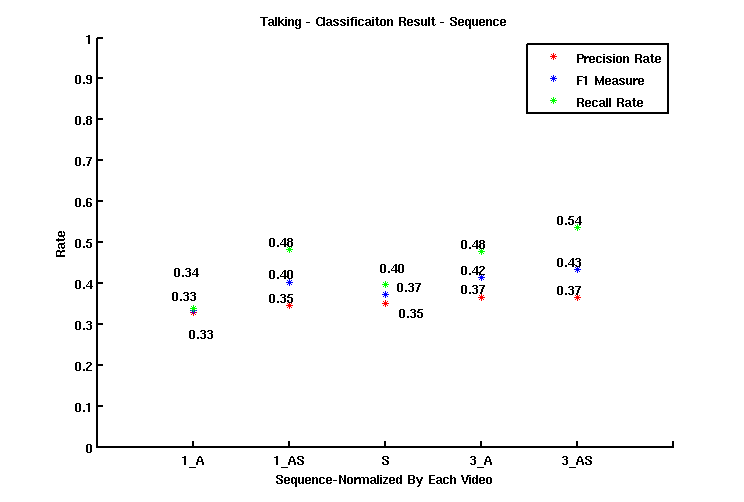
\includegraphics[width=\linewidth]{imgs/Result_Talking_Sequence.png}
  \caption{Class Talking - Classification Result of Sequence - Sequence normalised by each video}
  \label{fig:RTS}
\end{minipage}%
\begin{minipage}{.5\textwidth}
  \centering
  \captionsetup{justification=centering,margin=1cm}
  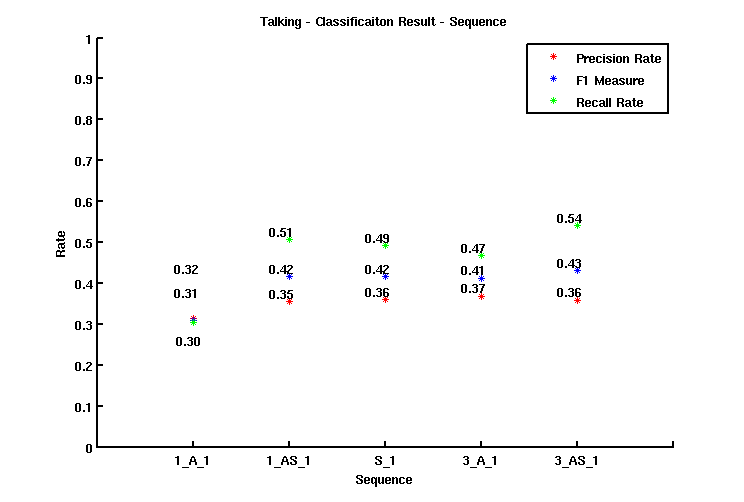
\includegraphics[width=\linewidth]{imgs/Result_Talking_Sequence_1.png}
  \caption{Class Talking - Classification Result of Sequence - Sequence NOT normalised by each video}
  \label{fig:RTS1}
\end{minipage}
\end{figure}
\newline
Average F1 score in figure \ref{fig:RTS} is 0.39, which is much higher than 0.2240 in figure \ref{fig:RES}. Also F1 score in figure \ref{fig:RTS1} is 0.398, which is also better than 0.216 in figure \ref{fig:RES1}. According to two above reasons, the classification of talking is better than eating. Compare figure \ref{fig:RES} and \ref{fig:RTS1}, it easy to find that there is not much increase on average recall rate but average precision rate of talking is much better than talking. It means classifier is better recognise not taking than not eating. This is the main reason why classification of talking is better than eating. In classify talking, there is an obvious increase of using 3\_A and there is a small increase on using 1\_AS and 3\_AS. From observation above, it seems appearance feature has a positive influence in classifier talking sequence. Compare figure \ref{fig:RTS} and \ref{fig:RTS1}, the F1 score in both figure is very similar, again it support the hypothesis that there is not much influence whether normalise data by each video. However, F1 score of S\_1 in figure \ref{fig:RTS1} is better than F1 score of S in figure \ref{fig:RTS}.
\begin{figure}[ht]
\centering
\begin{minipage}{.5\textwidth}
  \centering
  \captionsetup{justification=centering,margin=1cm}
  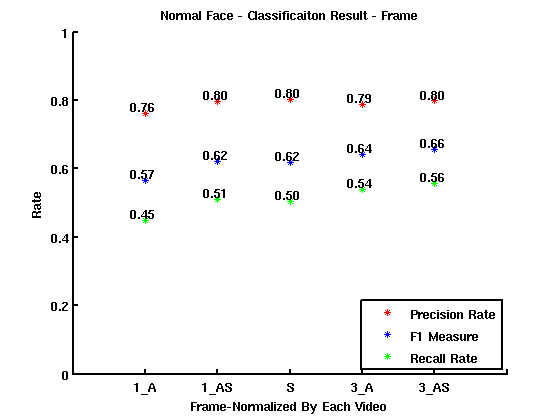
\includegraphics[width=\linewidth]{imgs/Result_NormalFace_Frame.png}
  \caption{Class Normal Face - Classification Result of Frame - Frame normalised by each video}
  \label{fig:RNF}
\end{minipage}%
\begin{minipage}{.5\textwidth}
  \centering
  \captionsetup{justification=centering,margin=1cm}
  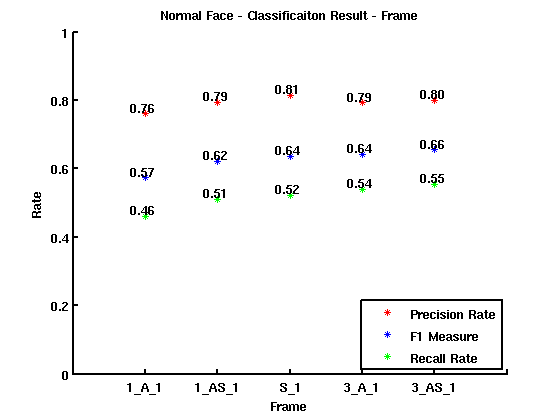
\includegraphics[width=\linewidth]{imgs/Result_NormalFace_Frame_1.png}
  \caption{Class Normal Face - Classification Result of Frame - Frame NOT normalised by each video}
  \label{fig:RNF1}
\end{minipage}
\end{figure}
\newline
The best classification result is classify normal face, it is much better than classify eating and talking. In both figure \ref{fig:RNF} and \ref{fig:RNF1}, the average recall rate is 0.51, precision rate is 0.79, and F1 score is 0.62. For normal face, the precision rate is higher than recall rate, which is different from classification result of eating and talking. From all frame classification result, figure \ref{fig:REF}, \ref{fig:REF1}, \ref{fig:RTF}, \ref{fig:RTF1},\ref{fig:RNF}, \ref{fig:RNF1}, comparing F1 score, it easy to see that using shape and appearance feature is always better than using just appearance feature and using 3-block appearance feature is always better than 1-block appearance feature.
\begin{figure}[ht]
\centering
\begin{minipage}{.5\textwidth}
  \centering
  \captionsetup{justification=centering,margin=1cm}
  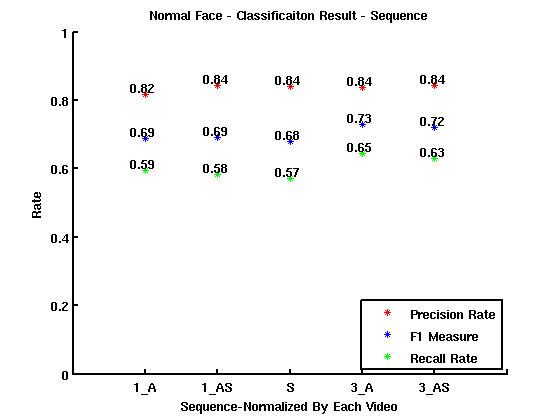
\includegraphics[width=\linewidth]{imgs/Result_NormalFace_Sequence.png}
  \caption{Class Normal Face - Classification Result of Sequence - Frame normalised by each video}
  \label{fig:RNS}
\end{minipage}%
\begin{minipage}{.5\textwidth}
  \centering
  \captionsetup{justification=centering,margin=1cm}
  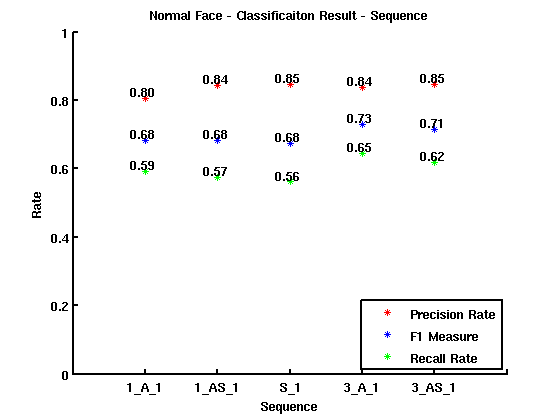
\includegraphics[width=\linewidth]{imgs/Result_NormalFace_Sequence_1.png}
  \caption{Class Normal Face - Classification Result of Sequence - Frame NOT normalised by each video}
  \label{fig:RNS1}
\end{minipage}
\end{figure}
\newline
In figure \ref{fig:RNS} and figure \ref{fig:RNS1}, average precision rate is 0.84, F1 score is 0.7, and recall rate is 0.605. There is 0.1 increase in F1 score comparing to frame classification result of normal face. The performance of using  S in figure \ref{fig:RNS} and \ref{fig:RNS1} is the worst among using different features, which is different from classify eating and talking. The best F1 score is obtained by using 3-block appearance feature and shape feature. It seems appearance feature is good for classifying normal face, but somehow had negative influence on classifying eating and talking. This may explain the reason why, using shape in classifying eating and talking performs relatively better than using appearance feature in classifying normal face.
\begin{figure}[ht]
\centering
\begin{minipage}{.5\textwidth}
  \centering
  \captionsetup{justification=centering,margin=1cm}
  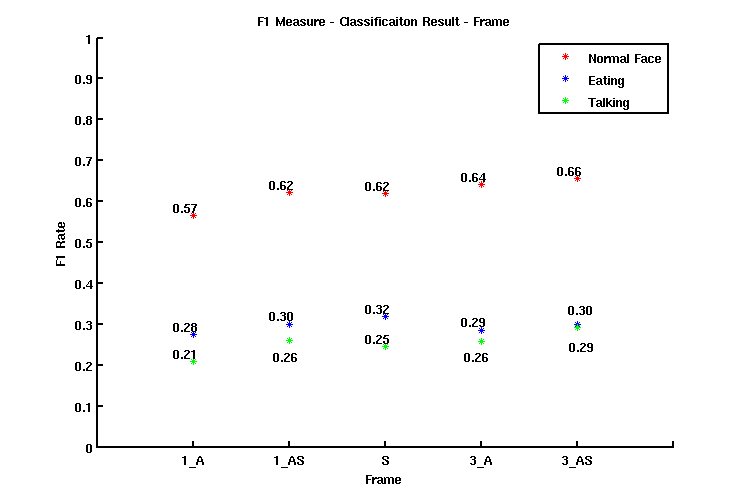
\includegraphics[width=\linewidth]{imgs/Result_F1_Frame.png}
  \caption{Three Class - Classification Result of frame - Frame normalised by each video}
  \label{fig:RFF}
\end{minipage}%
\begin{minipage}{.5\textwidth}
  \centering
  \captionsetup{justification=centering,margin=1cm}
  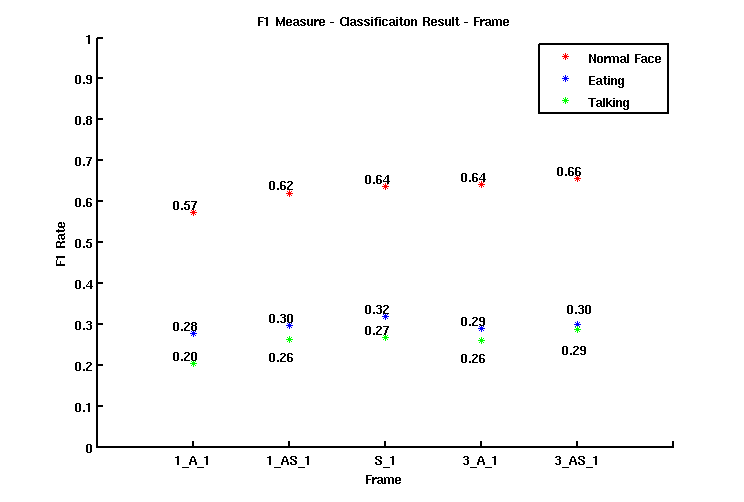
\includegraphics[width=\linewidth]{imgs/Result_F1_Frame_1.png}
  \caption{Three Class - Classification Result of frame - Frame NOT normalised by each video}
  \label{fig:RFF1}
\end{minipage}
\end{figure}
\newline
The frame classification result of three classes are shown in figure \ref{fig:RFF} and figure \ref{fig:RFF1}. Classification result from best to worst is normal face, eating, talking, according to F1 score. The process of normalise feature vector by each video does not increase classification result. However, using 3-block uniform pattern appearance feature which provide more appearance information has positive influence on classification result. By calculating the total F1 score of 10-group features, the best classification result is gained by using 3-block uniform pattern feature with shape feature. The worst classification is gained by using just 1-block appearance feature.
\begin{figure}[ht]
\centering
\begin{minipage}{.5\textwidth}
  \centering
  \captionsetup{justification=centering,margin=1cm}
  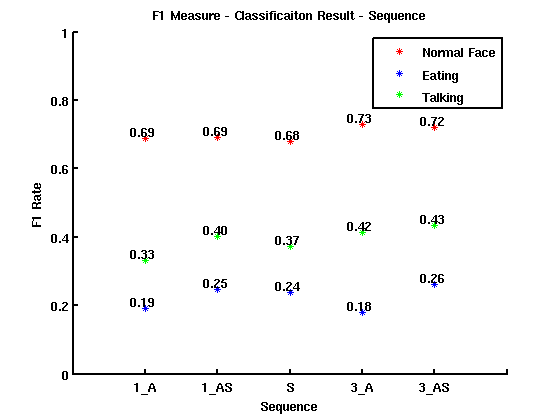
\includegraphics[width=\linewidth]{imgs/Result_F1_Sequence.png}
  \caption{Three Class - Classification Result of sequence - Frame nomalised by each video}
  \label{fig:RFS}
\end{minipage}%
\begin{minipage}{.5\textwidth}
  \centering
  \captionsetup{justification=centering,margin=1cm}
  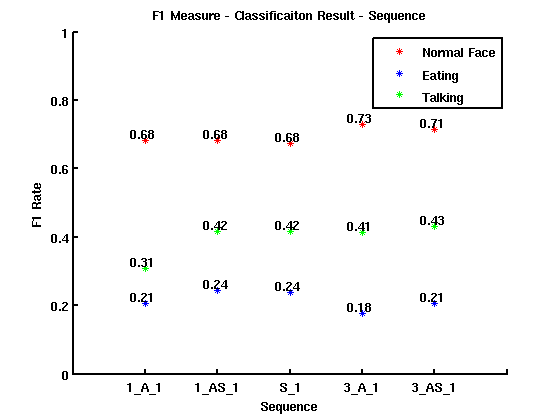
\includegraphics[width=\linewidth]{imgs/Result_F1_Sequence_1.png}
  \caption{Three Class - Classification Result of sequence - Frame NOT nomalised by each video}
  \label{fig:RFS1}
\end{minipage}
\end{figure}
\newline
For a sequence, the result of classify this sequence as a sequence of normal face, eating or talking is not directly classified by a classifier. It is calculated using majority voting from the classification result of frames. For example, the sequence is classified as a normal face if majority of frames are classified as normal face. Comparing result of classifying frame in figure \ref{fig:RFF} and sequence in figure \ref{fig:RFS}, the F1 score of normal face has a increase of 0.1, eating has a decrease of 0.08, talking has a increase of 0.14. The result of comparing figure \ref{fig:RFF1} and figure \ref{fig:RFS1} is almost the same. According to average F1 score of 10-group experiments, the best F1 score is gained by using 3-block appearance feature with shape feature, which is the same as frame classification result.

\begin{table}[ht]
\centering
\begin{tabular}{|c|c|c|c|}
\hline
\diagbox{Actual}{Predict}                             & \begin{tabular}[c]{@{}c@{}}Normal \\ Face\end{tabular}                            & Eating                                                                          & Talking                                                                         \\ \hline
\begin{tabular}[c]{@{}c@{}}Normal\\ Face\end{tabular} & \textbf{\begin{tabular}[c]{@{}c@{}}18271\\ (39.06\%)\end{tabular}} & \begin{tabular}[c]{@{}c@{}}7880\\ (16.85\%)\end{tabular}                        & \begin{tabular}[c]{@{}c@{}}6791\\ (14.52\%)\end{tabular}                        \\ \hline
Eating                                                & \begin{tabular}[c]{@{}c@{}}3156\\ (6.75\%)\end{tabular}                           & \textbf{\begin{tabular}[c]{@{}c@{}}3163\\ (6.76\%)\end{tabular}} & \begin{tabular}[c]{@{}c@{}}2425\\ (5.18\%)\end{tabular}                         \\ \hline
Talking                                               & \begin{tabular}[c]{@{}c@{}}1387\\ (2.97\%)\end{tabular}                           & \begin{tabular}[c]{@{}c@{}}1304\\ (2.79\%)\end{tabular}                         & \textbf{\begin{tabular}[c]{@{}c@{}}2400\\ (5.13\%)\end{tabular}} \\ \hline
\end{tabular}
\caption{Confusion Matrix-Frame-3\_AS}
\label{tab:CMF}
\end{table}
 Table \ref{tab:CMF} is an example of confusion matrix of frame using 3-block appearance feature with shape feature, more confusion matrix are in the appendix. From the table we can see, there are $48.78\% $ of frames are classified as normal face, $26.40\% $ are classified as Eating, $24.83\% $ are classified as talking.
\begin{table}[ht]
\centering
\begin{tabular}{|l|l|l|l|}
\hline
\diagbox{Actual}{Predict}                             & \begin{tabular}[c]{@{}c@{}}Normal\\ Face\end{tabular}                           & Eating                                                                       & Talking                                                                        \\ \hline
\begin{tabular}[c]{@{}c@{}}Normal\\ Face\end{tabular} & \textbf{\begin{tabular}[c]{@{}c@{}}538\\ (45.13\%)\end{tabular}} & \begin{tabular}[c]{@{}c@{}}162\\ (13.59\%)\end{tabular}                      & \begin{tabular}[c]{@{}c@{}}171\\ (13.35\%)\end{tabular}                        \\ \hline
Eating                                                & \begin{tabular}[c]{@{}c@{}}48\\ (4.03\%)\end{tabular}                           & \textbf{\begin{tabular}[c]{@{}c@{}}37\\ (3.1\%)\end{tabular}} & \begin{tabular}[c]{@{}c@{}}29\\ (2.43\%)\end{tabular}                          \\ \hline
Talking                                               & \begin{tabular}[c]{@{}c@{}}50\\ (4.30\%)\end{tabular}                           & \begin{tabular}[c]{@{}c@{}}45\\ (3.78\%)\end{tabular}                        & \textbf{\begin{tabular}[c]{@{}c@{}}112\\ (9.40\%)\end{tabular}} \\ \hline
\end{tabular}
\caption{Confusion Matrix-Sequence-3\_AS}
\label{tab:CMS}
\end{table}
\newline
Table \ref{tab:CMS} is an example of confusion matrix of sequence using 3-block appearance feature with shape feature, more confusion matrix are in the appendix.The approximate percentage of sequences classified as normal face, eating, talking is $54\% $, $21\% $, $25\% $. Comparing to frames, an obvious change is that there is increase in normal face and there is a decrease in eating. It seems, there are more sequence with low number of frames in normal face than eating. This hypothesis was proven and the evidence is in next subsection. 
\subsection{Data and Analysis}
\begin{table}[h]
\centering
\captionsetup{justification=centering,margin=4cm}
\begin{tabular}{|c|c|c|c|}
\hline
      & \begin{tabular}[c]{@{}c@{}}Normal\\ Face\end{tabular} & Eating & Talking \\ \hline
1-10  & 322         & 32     & 90      \\ \hline
11-20 & 122         & 17     & 45      \\ \hline
21-30 & 117         & 18     & 25      \\ \hline
30-40 & 91          & 8      & 16      \\ \hline
41-50 & 35          & 3      & 7       \\ \hline
50+   & 184         & 36     & 24      \\ \hline
\end{tabular}
\caption{The left column is frame number, first row is the class name. This table shows the number of sequences with frame number in the certain range.}
\label{tab:DAFNS}
\end{table}
In order to find out why the classification result is not good, and there is a big difference from classification result of frames and sequences. We statistical count the frame number of each sequence(shown in table \ref{tab:DAFNS}). In table \ref{tab:DAFNS}, the number of sequences with frame number between 1 to 10 is very large especially for normal face. Eating contains less low frame number sequence, this may be the reason there is a big difference in frame confusion matrix and sequence confusion matrix especially for normal face and eating. As the number of image sequence is so imbalance, majority voting strategy does not improve the result of sequence. Table \ref{tab:DAFNS2} in appendix gave a detail number of sequences with frame number  from 1 to 10. It also shows the imbalance of testing data.
\subsection{Examples of Wrong Classification}
\begin{figure}[ht]
\centering
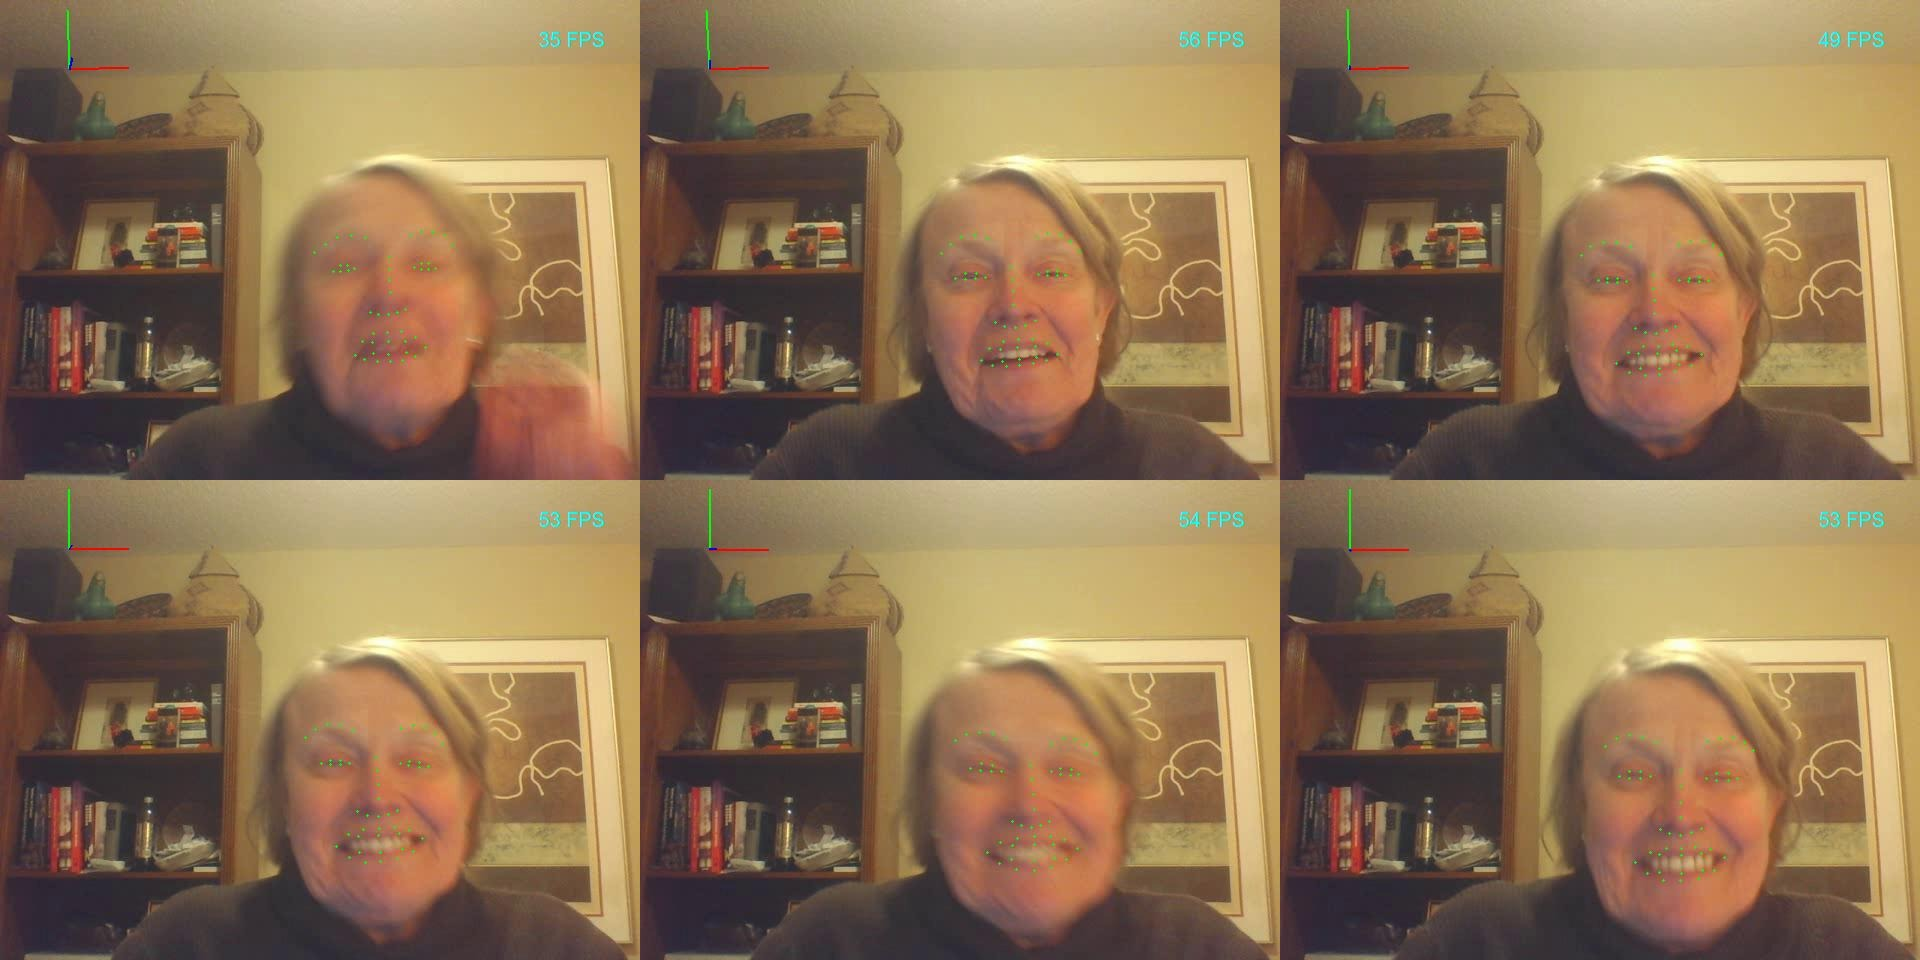
\includegraphics[width = \textwidth]{imgs/Wrong_NF00.jpg}
\caption{Wrong classification of normal face. Classification Result: [3 3 3; 3 3 1]}
\label{fig:EXPNF}
\end{figure}
In this dataset, there is no smiling label and smiling is treated as normal face. Such as the example shown in figure \ref{fig:EXPNF}, the subject smiles and the action of mouth region could be classified into wrong class.
\begin{figure}[ht]
\centering
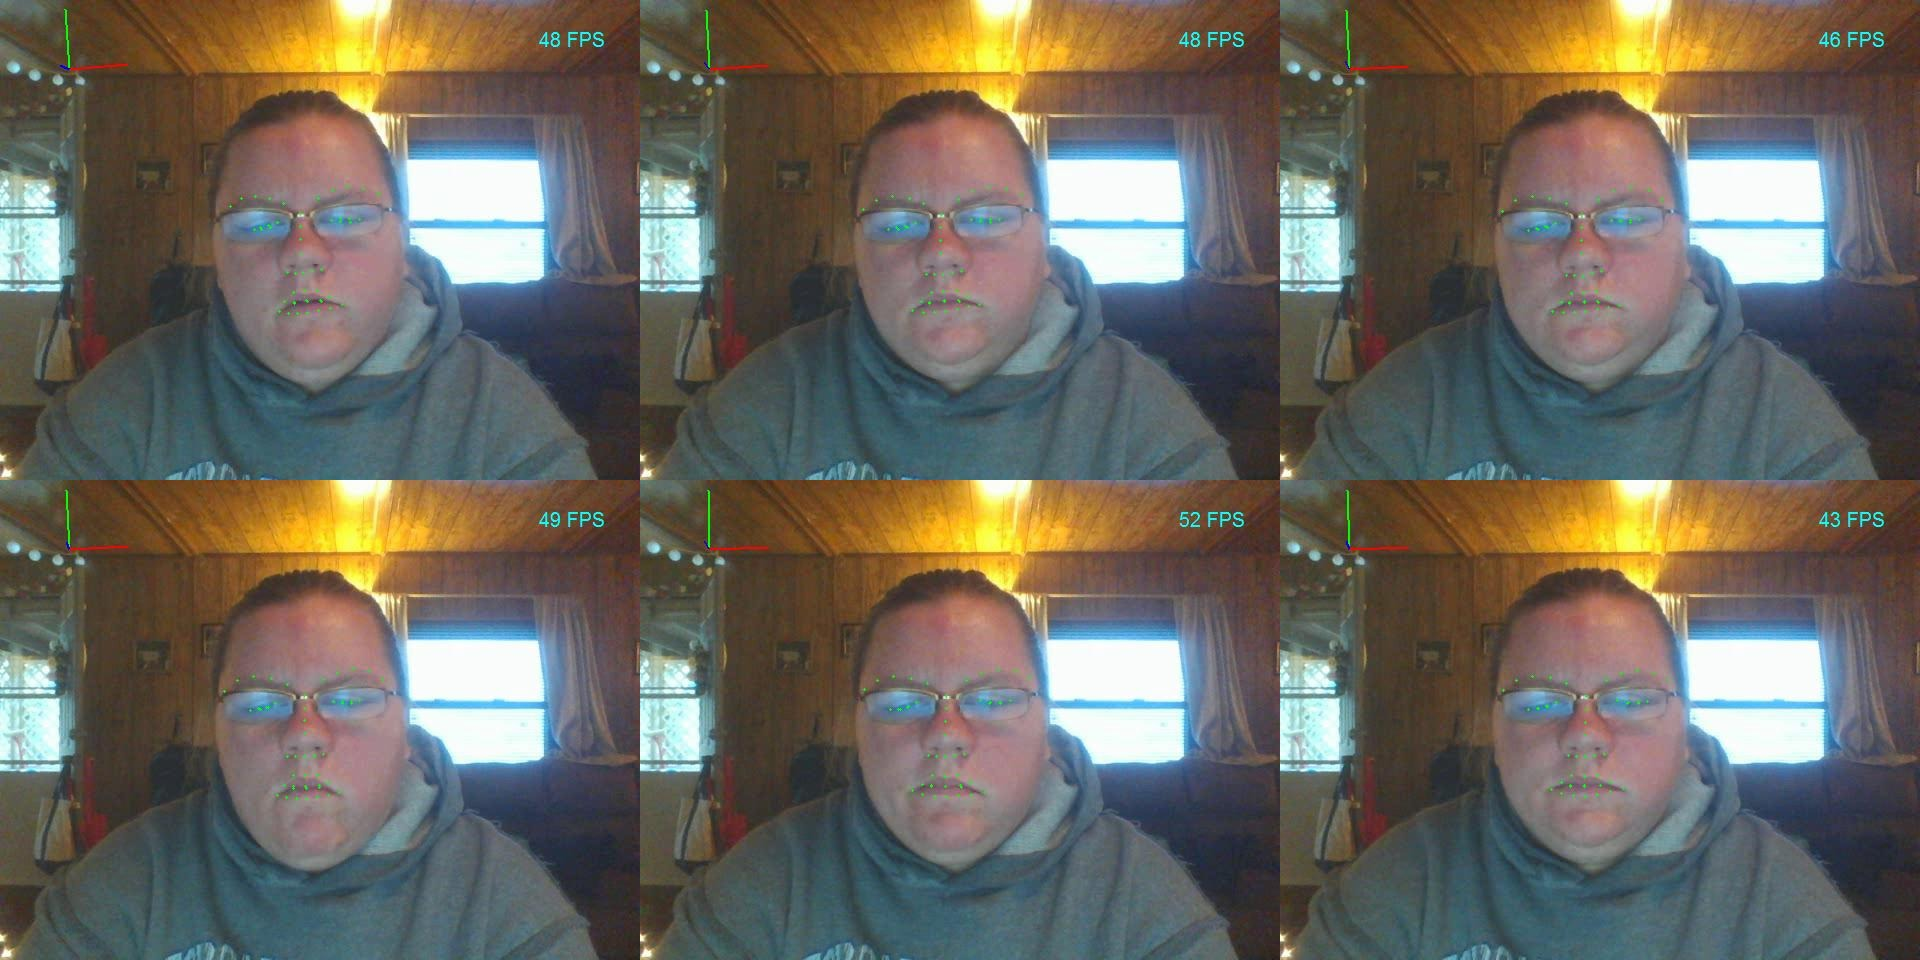
\includegraphics[width = \textwidth]{imgs/Wrong_E00.jpg}
\caption{Wrong classification of normal face. Classification Result: [1 1 1; 3 1 2]}
\label{fig:EXPE}
\end{figure}
\newline
Figure \ref{fig:EXPE} gave an example of wrong classification of eating. As you can see subject's mouth barely moves while chewing. And usually for a long video of eating sequence, it will contain many images of normal face as the subject would not keep eating and chewing without rest. The state of eating is always changing, it's more like a continuous states instead of a constant state of eating. SVM is good for modelling this type of state changing. Hidden Markov Model or long-term memory neural network may be better in modelling state changing. However, as database does not contain small sequence which just contain one complete eating. The time for doing this project is limited, it is  impossible to label the videos by hands.
\begin{figure}[ht]
\centering
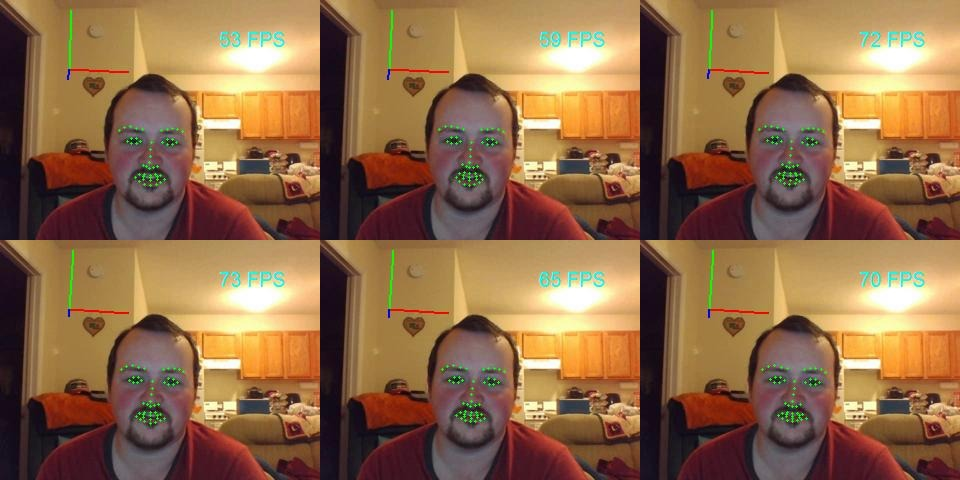
\includegraphics[width = \textwidth]{imgs/Wrong_T00.jpg}
\caption{Wrong classification of Talking. Classification Result: [1 3 3; 1 1 1]}
\label{fig:EXPT}
\end{figure}
\newline
Figure \ref{fig:EXPT} is a complete sequence of talking. Just by observing the image, it is hard to tell that the subject is talking. Four of the frames are classified as normal face, and these images looked very similar as normal face.
\paragraph{Conclusion}
Video set used in this project is recorded in uncontrolled environment, the condition of each video is different. The lighting condition ,head moving, resolution of frames and the proportion of face inside the frame are very different. The number of each sequence is very different, it contains too many short sequence which should be filtered while using the data. In conclusion,more process should be done for filtering the sequences for classification step. Normal face frame may be not suitable for detection in this image as normal face contain many action such as smiling, this would increase the difficulty of classifying normal face from other facial expressions. The model may be not good for expressing eating and talking.